\subsection{{\bf Comparison on Name Prediction (JS)}}
\label{empirical-rq1}

%\begin{table}[t]
%	\caption{RQ1. Comparative Study on Variable Name Prediction.}
%	\begin{center}
%		\small
%		\renewcommand{\arraystretch}{1} 
%		\begin{tabular}{p{2cm}<{\centering}|p{2cm}<{\centering}|p{2cm}<{\centering}}
%			\hline
%		                & Local Variables & All Variables\\
%			\hline
%			JSNice~\cite{JSNice2015}      &                 &         \\
%			JSNaughty~\cite{JSNaughty2017}   &                 &         \\
%                       JSNeat~\cite{icse19}      & 0.64            & 0.66    \\
%			\hline
%			{\tool}     & 0.67            & 0.76    \\
%			\hline
%		\end{tabular}
%		\label{RQ1-result}
%	\end{center}
%\end{table}

\begin{figure}[t] %[thbp]
\begin{center}
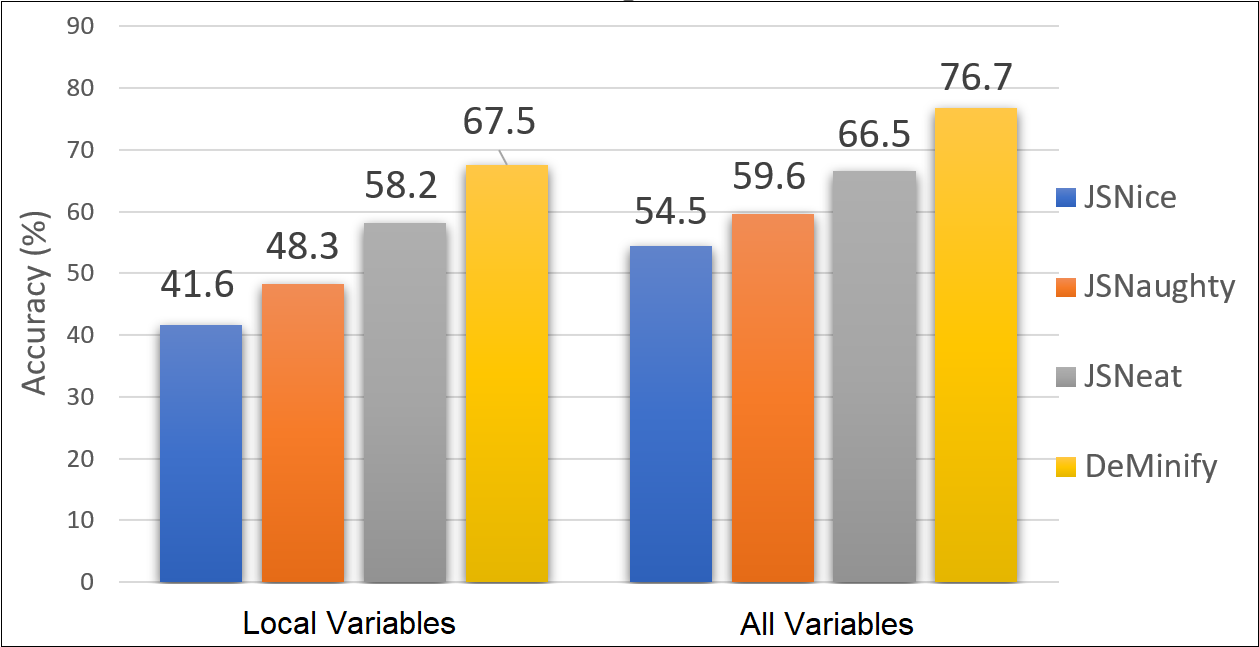
\includegraphics[width=3.2in]{figures/name-prediction-result-2}
\vspace{-8pt}
\caption{RQ1. Top-1 Accuracy on Variable Name Prediction}
\label{name-prediction-result}
\end{center}
\end{figure}





%In this study, we evaluate {\tool}'s accuracy and compare it with the
%state-of-the-art approaches in variable name prediction for minified
%code.
%In this study, we evaluate {\tool} in variable name prediction.
As seen in Figure~\ref{name-prediction-result}, for all variables in
minified code, {\tool} achieves high top-1 accuracy of {\bf 76.7\%}:
in 76.7\% of the cases, it can recover the correct variable names with
a single prediction. The relative improvements in top-1 accuracy for
all variables over JSNice, JSNaughty, and JSNeat are {\bf 40.7\%,
  28.7\%}, and {\bf 15.3\%}, respectively. The absolute improvements
in top-1 accuracy over the state-of-the-art approaches are from
10.2\%--22.2\%.

Considering only local variables, in {\bf 67.5\%} of them, {\tool}
correctly predicts their original names with a single result. The
relative improvements in top-1 accuracy in recovering local variables'
names over JSNice, JSNaughty, and JSNeat are {\bf 62.2\%, 39.8\%}, and
{\bf 15.9\%}, respectively. The absolute improvements in top-1
accuracy over the state-of-the-art approaches are from 9.3\%--25.9\%.

\begin{table}[t]%[thbp]
  \caption{RQ1. Comparison on Variable Name Prediction}
  \vspace{-8pt}
	\begin{center}
		\small
		\renewcommand{\arraystretch}{1} \begin{tabular}{|p{1.9cm}<{\centering}|p{0.65cm}<{\centering}|p{0.65cm}<{\centering}|p{0.65cm}<{\centering}|p{0.65cm}<{\centering}|p{0.65cm}<{\centering}|p{0.65cm}<{\centering}|}
			
			\hline
                       & \multicolumn{2}{c|}{Top-1}         & \multicolumn{2}{c|}{Top-3}         & \multicolumn{2}{c|}{Top-5} \\
			\hline
                       & Local & All & Local & All & Local & All  \\ 
			\hline
		        JSNice~\cite{JSNice2015} &  41.6    & 54.5  & 52.2 &    63.0   & 59.5      &   67.8    \\
			JSNaughty~\cite{JSNaughty2017}  &   48.3   &  59.6    &  59.8    &  69.7    &  66.3    &   75.0    \\
			JSNeat~\cite{icse19}  &   58.2   &  66.5    &  65.3    & 75.4     &  71.6    & 80.1     \\
			\hline
			{\bf {\tool}} & 67.5 & 76.7 & 75.4 & 84.3 & 82.1 & 90.2 \\
			\hline
		\end{tabular}
		\label{name-JS-result}
	\end{center}
\end{table}

As seen in Table~\ref{name-result} and Table~\ref{name-JS-result}, the
results are consistent for both languages. The relative improvements
are with same trends in comparison with the baselines.

%which is not as powerful as the advanced neural network
%GCNmf~\cite{GCNmf}.


%1. On both local variables and all variables, {\tool} performs XXX\%
%better than the baselines.

%2. JSNeat uses information retrieval techniques to find the possible
%variable names based on the training data. {\tool} can perform better
%because sometimes it is hard to find similar variable names with
%similar variable relationships, and sometimes the same variable names
%may have different variable relationships. JSNeat cannot perform well
%in these cases, but {\tool} can still work as designed.

%3. JSNice uses conditional random field models to predict variable
%names based on dependency graphs. {\tool} can outperform {\tool} by
%XX\% because {\tool} uses combine graph from relation graph and
%TDG. The combined graphs contain more detailed information between
%variables compared with dependency graphs.

%4. JSNaughty regards the name prediction problem as the translation
%problem. {\tool} can outperform JSNaughty XX\% because different
%minification tools can provide different minified variable names for
%the same source code, but {\tool} regards the minified variable names
%as missing features in GCNmf. In this case, the minified variable
%names will not influence the performance of {\tool}, but it will
%influence JSNaughty performance.
